% Chapter Template

\chapter{Signal Region Optimisation} % Main chapter title

\label{Chapter5} % Change X to a consecutive number; for referencing this chapter elsewhere, use \ref{ChapterX}

\lhead{Chapter 5. \emph{Signal Region Optimisation}} % Change X to a consecutive number; this is for the header on each page - perhaps a shortened title

%----------------------------------------------------------------------------------------
%	SECTION 1
%----------------------------------------------------------------------------------------
%\section{Strategy in Run 1}

In order to maximise sensitivity to a wide range of signal models 
the final analysis bins must be carefully chosen. 
In Run 1 a flat $\alphat > 0.55$ requirement was used. However, 
while the \alphat variable is highly adept at removing the
QCD multijet background it may not be optimal for distinguishing 
signal from the remaining background. Additionally, each bin can have
only one \alphat (and therefore \mht) threshold and no advantage 
may be taken of the shape. Finally, each jet category has the same 
\alphat threshold per \scalht bin. Higher jet multiplicities lead to 
lower \alphat values and so more flexibility is desirable. 
In this section when the \scalht bin for each particular jet and btag 
category is considered this will be denoted as \scalhtcat.


\section{Strategy for Run 2}

The trigger strategy has been optimised to allow lower \alphat thresholds in each bin. 
This deals with the QCD multijet background. Sensitivity may then be maximised
by using a new discriminating variable such as \mht to conduct a shape analysis in each bin.
In order to retain some control in data a requirement of 10 events is made
on control counts for the highest new variable threshold.

In each \scalhtcat bin the normalisation and systematics are set by the control samples
and closure tests described in Section~\ref{sec:bkgd-est}. The scale of the event is
thus fully controlled in data. Investigations are underway for how the shapes 
and systematics can be found using the shape in the control regions. Given the low
counts in the tails some kind of fit and extrapolation would be required.
Alternatively the systematics may be estimated entirely from MC by varying the main 
sources of systematic uncertainty and finding the effect on the shape.




\section{Results}

The results considered below consider a simplified approach where bins in the NV dimension are given a single correlated systematic decided by the closure test. This therefore allows an easy comparison between different variables and the gain from adding bins below the furthest threshold.






% \begin{figure}
% \centering
%     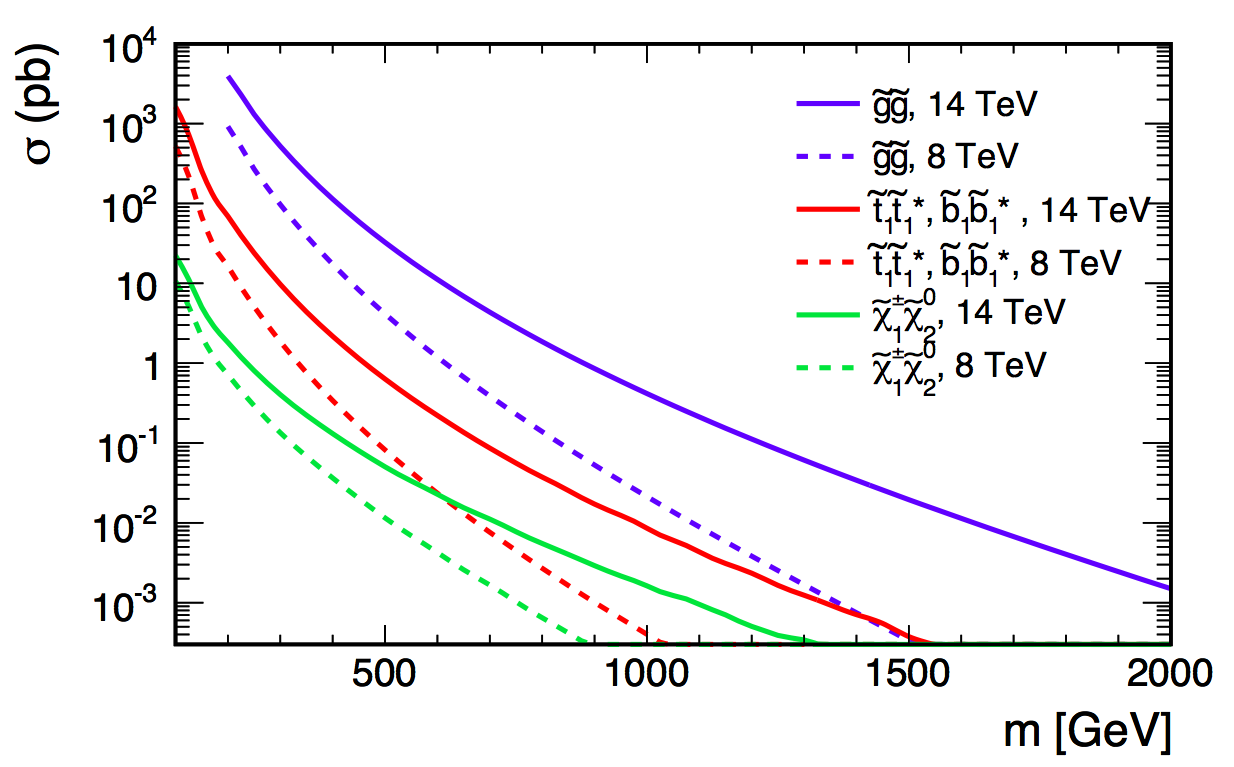
\includegraphics[width=0.7\textwidth]{Figures/snowmass.png}
%   \caption{SUSY production cross sections at 14 TeV compared with 8TeV}
%   \label{snow}
% \end{figure}


% \subsection{Automated Binning}
%
% To determine the binning in the NV an automated procedure is used. Initially this is run for each signal model separately and works as follows. 
% \begin{enumerate}
% \item To ensure the analysis remains data driven the NV threshold is chosen such the number of events in the control samples (not split in btags) for the relevant backgrounds is sufficient to carry out closure tests. This threshold is then used as an upper bound for the NV binning ($NV_{closure}$). 
%   \item This the systematic error is taken from closure tests. This will be \scalhtcat dependant for the case of correlated NV bins or also NV dependant if the NV bins are decorrelated.  	
%   \item The signal and background counts integrated from each NV threshold to $\infty$ are found.
%   \item The systematic error is added in quadrature to the statistical error determined from the transfer factor from the control region to the signal region.
%   \item The significance is the found for every possible NV cut value using the asymptotic formula considering data counts given by background plus signal contribution and the background only prediction with the uncertainty determined above. This is truncated at $NV_{closure}$.
%   \item The significance is then smoothed to remove fluctuations and the maximum is assigned as the highest lower bin threshold.
%   \item The procedure is repeated integrating up to the lower bin threshold found in the previous step. A minimum bin width is enforced to minimise bin migration.
%   \item The procedure stops when the significance is below a predetermined threshold.
% \end{enumerate}
% \begin{table}[h!]
%   \caption{\alphat and (effective) \mht thresholds per \scalht bin.\label{tab:alphat-thresholds}. For the $>$800 bin there is a direct \mht rather than \alphat requirement}
%   \centering
%   \footnotesize
%   \begin{tabular}{ lccccccc }
%     \hline
%     \hline
%     \scalht      & 200--250   & 250--300   & 300--350  & 350--400  & 400--800 \\ & $>$800       \\
%     \hline                                                                     
%     \alphat      & 0.65       & 0.60       & 0.55      & 0.53      & 0.52     \\  & 0         \\
%     "Min \mht"   & $\sim$128  & $\sim$138  & $\sim$125 & $\sim$133 & $\sim$137 \\  & 130 \\
%     \hline
%     \hline
%   \end{tabular}
% \end{table}
%
% To ensure the same bins are used for all signal models a representative selection of models are used to determine the optimal binning for each \scalhtcat bin. The model with the highest exclusion in each bin then determines the binning. This is done for every \scalhtcat bin and a standard binning is found for all models.
% \subsection{Strategies}
%
% There are several possible strategies for binning and utilising the data in each \scalhtcat bin. The most similar approach to the previous strategy is simply to choose NV thresholds (per \scalht) which map closely to the \alphat requirements used in Run 1 (S0). Following from this is to run the optimisation procedure described below and use the last NV threshold in each \scalhtcat bin (S1). In these cases systematics are detemined via the closure tests in exactly the same way as for Run 1.
%
% The last two strategies take advantage of the full range of the NV. The more conservative approach is to determine uncorrelated systematics in the NV dimension via closure tests and use these to determine bin thresholds per NV value. These systematics are used in the optimisation and the likelihood is fully binned with uncorrelated systematics along the NV dimension (S2). This has the advantage of remaining purely data driven. Finally, a shape analysis can be used. In this case there is no need for optimisation. The normalisation systematic is the same as for S0 and S1 (fully determined by data) but templates generated using Monte Carlo in the signal region for each dominant systematic source are used as the shape systematics for each background source along the NV dimension.
